\newcommand{\be}{\begin{equation}}
  \newcommand{\ee}{\end{equation}}
\newcommand{\ba}{\begin{eqnarray}}
  \newcommand{\ea}{\end{eqnarray}}

\documentclass{beamer}

\usepackage{beamerthemesplit,amsmath,amssymb,latexsym,graphicx,hyperref}

\title{Curve fitting}
\author{Ramkumar R}
\date{\today}

\begin{document}

\frame{\titlepage}

\section[Outline]{}
\frame{\tableofcontents}

\section{Probability 101}
\frame
{
  \begin{itemize}
  \item Random variables
  \item Probability functions
    \begin{itemize}
    \item Discrete PMF
    \item CDF
      \be
      F_X(x) = Prob\{X\leq x\}
      \ee
    \item PDF
      \be
      f_X(x) = F'(x)
      \ee
    \end{itemize}
  \end{itemize}
}
\frame
{
  \frametitle{Moments}
  \begin{itemize}
  \item Central moment | $\langle(x-\mu)^{m}\rangle = \langle(x- \langle x \rangle)^{m}\rangle$
    \begin{itemize}
    \item Zeroth and First | 1 and 0
    \item Second | Variance $\sigma^{2} = \langle (x- \langle x \rangle)^{2} \rangle = \langle x^{2} \rangle - \langle x \rangle ^{2}$
    \item Third and Fourth | Skewness and Kurtosis
    \end{itemize}
  \item Non-central moment | $\langle X^{m} \rangle$
  \end{itemize}
}
\section{Distributions}
\subsection{Gaussian (Normal)}
\frame
{
  \frametitle{Gaussian (Normal)}
  \begin{center}
  \resizebox{75mm}{!}{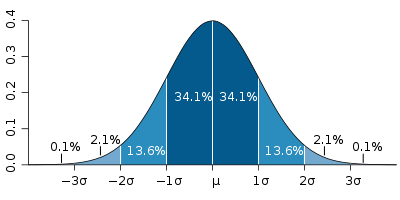
\includegraphics{img/gaussian.png}}
  \end{center}
  \be
  f_X(x) = \frac{1}{\sigma \sqrt{2\pi}} \exp \left\{ -\frac{(x-\mu)^2}{2\sigma^2}\right\}
  \ee
}
\subsection{Chi-square}
\frame
{
  \frametitle{Chi-square PDF}
  \be
  Q=\sum_{i=1}^{k} \, X_i^2
  \ee
  \be
  f_Q(x;k) =
  \begin{cases}
    \frac{1}{2^{k/2} \Gamma(k/2)} x^{k/2\,-\,1} e^{-x/2} & \ ;\ x\geq0 \\
    0 & \ ;\ x<0
  \end{cases}
  \ee

  where $X_i$'s are normallly distributed random variables with 0 mean and variance 1.
}
\frame
{
  \frametitle{Chi-square CDF}
  After integration, we get the Chi-square CDF in terms of an lower incomplete $\gamma$ function defined as \\
  \be
  \gamma(s,x)= \int_0^x t^{s-1}e^{-t} \, dt
  \ee
  Then the Chi-square CDF equals
  \be
  \frac{\gamma(\frac{k}{2},\frac{\chi^{2}}{2})}{\Gamma(\frac{k}{2})}
  \ee
}
\section{Curve Fitting}
\subsection{Introduction}
\frame
{
  \frametitle{What does curve fitting mean?}
  \begin{itemize}
  \item Fitting data to a model with adjustable parameters
  \item Design figure-of-merit function
  \item Obtain best fit parameters by adjusting parameters to achieve min in merit function
  \item More details to take care of
    \begin{itemize}
    \item Assess appropriateness of model; goodness-of-fit
    \item Accuracy of parameter determination
    \item Merit function may not be unimodal
    \end{itemize}
  \end{itemize}
}
\subsection{Specific fits}
\frame
{
  \frametitle{Least squares fitting}
  Maximizing the product
  \be
  P \varpropto \prod_{i=1}^{N}{\exp \left[- \frac{1}{2} \left(\frac{y_i-y_{i(t)}}{\sigma} \right)^2 \right]} \Delta y
  \label{deriveChiSq}
  \ee
  ie. Minimizing its negative logarithm
  \be
  \left[\sum_{i=1}^{N}\frac{[y_{i}-y_{i(t)}]^2}{2\sigma^2}\right]-N\log \Delta y
  \ee
  Minimizing this sum over $a_1, a_2, .. a_M$, we get the final form:
  \be
  \sum_{i=1}^N [y_i-y_{i(t)}]^2
  \ee
}
\frame
{
  \frametitle{Chi-square fitting}
  Modifying equation \ref{deriveChiSq} to replace the $\sigma$ by $\sigma_i$ and going through the same process, we get
  \be
  \chi^2 = \sum_{i=1}^N \left(\frac{y_i-y_{i(t)}}{\sigma_i}\right)^2
  \ee
  where
  \be
  y_{i(t)} = f(a_1, a_2, .. a_M)
  \ee
  For models that are linear in the a's, however, it turns out that the probability distribution for different values of chi-square at its minimum can nevertheless be derived analytically, and is the chi-sqaure distribution for \texttt{N-M} degrees of freedom.
}
\section{Implementation}
\frame
{
  \frametitle{gnuplot}
  \begin{center}
    \texttt{gnuplot> fit f(x) `foo.data' u 1:2:3:4 via a, b}
  \end{center}
  \begin{itemize}
    \item Uses WSSR: Weighted Sum of Squared Residuals
    \item Marquardt-Levenberg algorithm to find parameters to use in next iteration
    \item After fitting, gnuplot reports \textit{stdfit}, the standard deviation of the fit
  \end{itemize}
}
\section{Credits}
\frame
{
  \begin{itemize}
  \item Numerical Receipies in C
  \item The gnuplot manual
  \item Miscellanous books on elementary probability
  \item Presentation created using \LaTeX{} and Beamer
  \end{itemize}
  \small
  Presentation source code available on \href{http://github.com/artagnon/authored}{github.com/artagnon/authored}
}
\end{document}
